\documentclass[10pt]{beamer}

\usetheme{metropolis}
\usepackage{appendixnumberbeamer}

\usepackage{booktabs}
\usepackage[scale=2]{ccicons}
\usepackage{graphicx}
\usepackage{pgfplots}
\usepgfplotslibrary{dateplot}
\usepackage{caption}
\usepackage{subcaption}
\usepackage{xspace}
\usepackage{hyperref,xcolor}
\usepackage{textpos}
\usepackage{appendixnumberbeamer}
\usepackage{makeidx}
\usepackage{verbatim}
\definecolor{winered}{rgb}{0.5,0,0}
\newcommand{\themename}{\textbf{\textsc{metropolis}}\xspace}


\defbeamertemplate*{background canvas}{bg}
{%
	\color{white}\vrule width\paperwidth height\paperheight% added bg color
}





\title{Bhabha Tracking Efficiencies}
%\subtitle{A modern beamer theme}
\date{09.08.2019}
\author{Martin Sobotzik}
\institute{Johannes Gutenberg-Universit\"at Mainz}
% \titlegraphic{\hfill
\includegraphics[height=1.5cm]{logo.pdf}}

\definecolor{darkblue}{rgb}{0,0,.5}
\hypersetup{pdftex=true, colorlinks=true, breaklinks=true, linkcolor=darkblue, menucolor=darkblue, pagecolor=darkblue, urlcolor=darkblue}


%citecolor={winered} %Gives errors when turned on
%allcolors={winered} %Gives errors when turned on

\begin{document}

\maketitle
%
\setbeamertemplate{frame footer}{}

%\section{Reproducing Plots}


\begin{frame}{Motivation}

\begin{itemize}	
	\item I am performing an analysis to estimate the tracking efficiency on phase 2 data
	\item The process I am considering is Bhabha events $\textrm{e}^+ \textrm{+e}^- \rightarrow \textrm{e}^+ \textrm{+e}^- $ 
	\item The definition of efficiency I am going to use is:

\end{itemize}
	\begin{equation*}
		\epsilon = \frac{\textrm{Number of Bhabha events with exactly 2 tracks}}{\textrm{Number of Bhabha events with 1 or more tracks}}
	\end{equation*}
	
	\begin{itemize}
		\item After selecting Bhabha events where at least one of the tracks was detected, one can look how many times the second one is found
		\item  This idea comes from some plots presented by Sam Cunliffe in previous  \href{https://confluence.desy.de/display/BI/ECL+Meetings?preview=/84320165/109161400/SCunliffe181123-ECL.pdf}{tracking and ECL} meetings.
	\end{itemize}





\end{frame}
	
	
\begin{frame}{Best Candidate Selection}
	
	\begin{textblock*}{\textwidth}(0cm,-4cm)
		\begin{center}	
			$\textrm{vpho} \rightarrow \textrm{ECL-Object(HclE)} + \textrm{ECL-Object(LclE)}$	
		\end{center}

	\end{textblock*}
	
	\begin{textblock*}{\textwidth}(0cm,-3.05cm)
		\scriptsize{		HcLE: particle with the higher cluster Energy; 	
		LclE: particle with the lower cluster Energy
}		
	\end{textblock*}

	
	
	
	\begin{textblock*}{1.2\textwidth}(-0.7cm,-2.8cm)
		

	
	
	\begin{itemize}
		
		\item $0.296706 < \theta_{\textrm{ECL Object}} < 2.61799 \rightarrow$ It has to hit the ECL
		\item Exactly two clusters with at least $3.5\,\textrm{GeV}$ per event and one cluster has to have at least $4.5\,\textrm{GeV}$
		\item $8\,\textrm{GeV} < \textrm{M}_{\textrm{vpho}} < 12\,\textrm{GeV}$
		\item $\textrm{nTracks} < 7$ 
		\item $\textrm{Total Energy in the ECL} < 15\,\textrm{GeV}$
						
		\end{itemize}

	\end{textblock*}


\begin{textblock*}{0.5\textwidth}(0cm,1cm)
	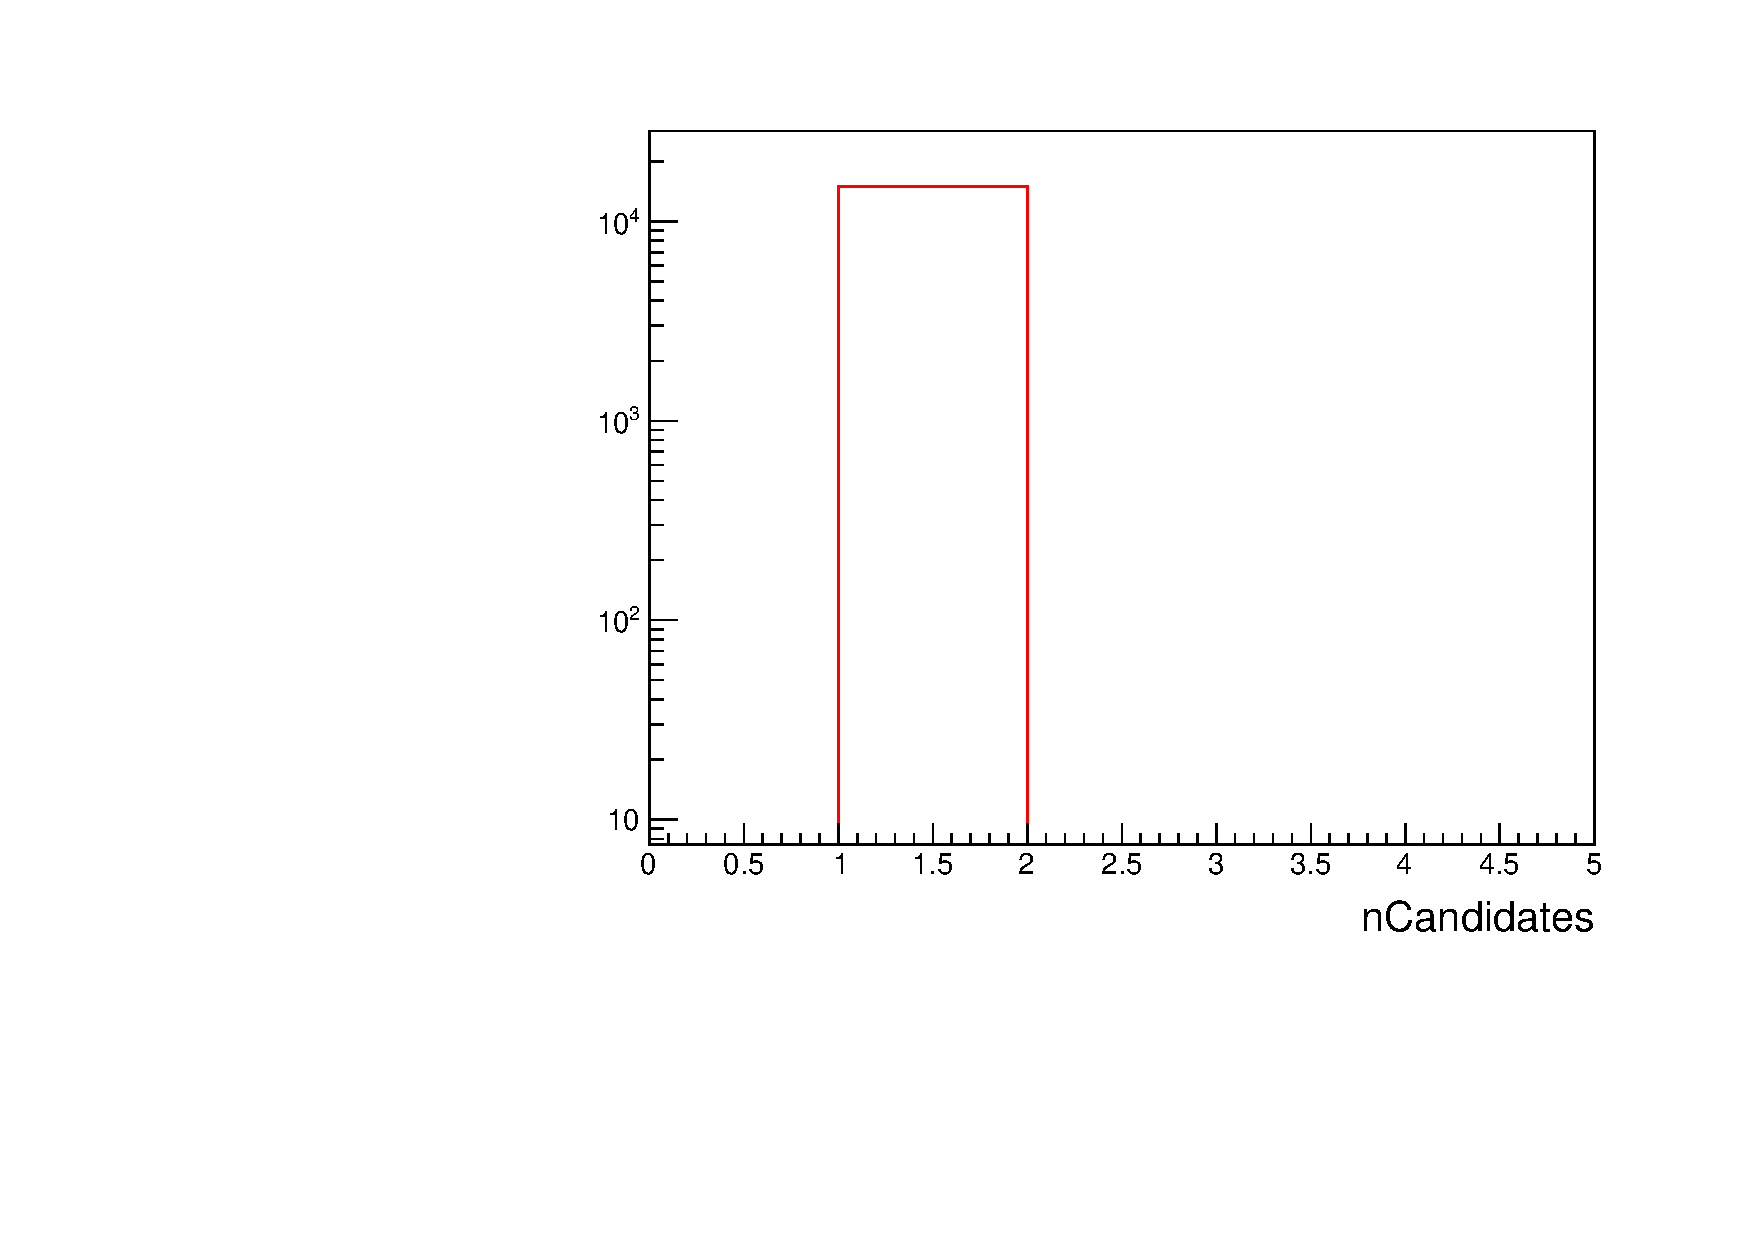
\includegraphics[width=4.5cm]{Plots/nCandMC}
\end{textblock*}


	
\begin{textblock*}{0.5\textwidth}(6cm,1cm)
	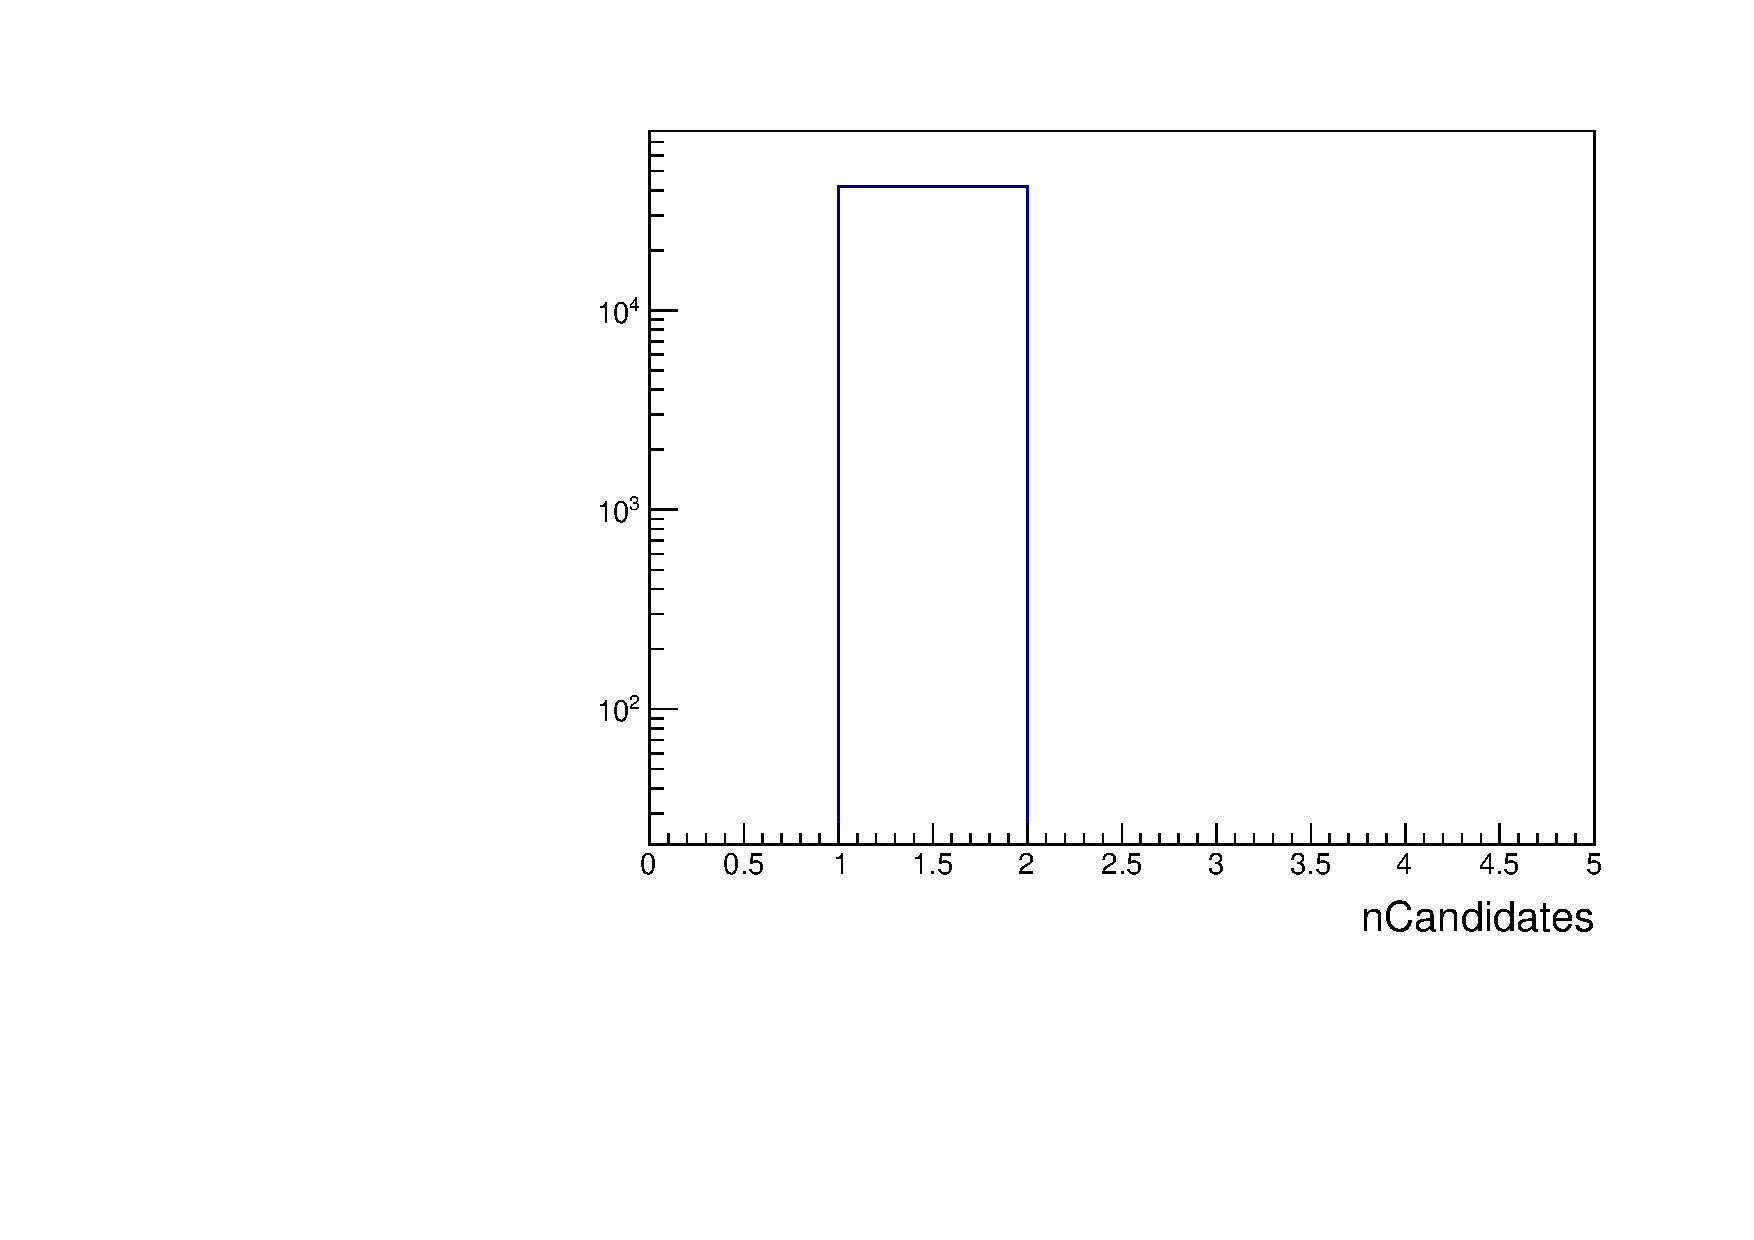
\includegraphics[width=4.5cm]{Plots/nCandData}
\end{textblock*}
	
	
\begin{textblock*}{0.5\textwidth}(1cm,1cm)
	\footnotesize
	\textcolor{red}{1 MC $\textrm{ee} \rightarrow \textrm{ee}$ File}
\end{textblock*}	
	
\begin{textblock*}{0.5\textwidth}(6.35cm,0.5cm)
	\footnotesize
	\textcolor{blue}{Phase 2 data}
	
	\textcolor{blue}{r02608/all/mdst/sub00/*.root}
\end{textblock*}	

	
	
	
\end{frame}


\begin{frame}{Bhabha Event Selection}

	\begin{figure}
		\centering
		\includegraphics<1>[width=\textwidth]{Plots/b2b_2}
	\end{figure}
	
\end{frame}
	
	
\begin{frame}{Bhabha Event Selection (Phase 2 data)}
	
	\begin{textblock*}{0.5\textwidth}(0cm,-3cm)
		\centering
		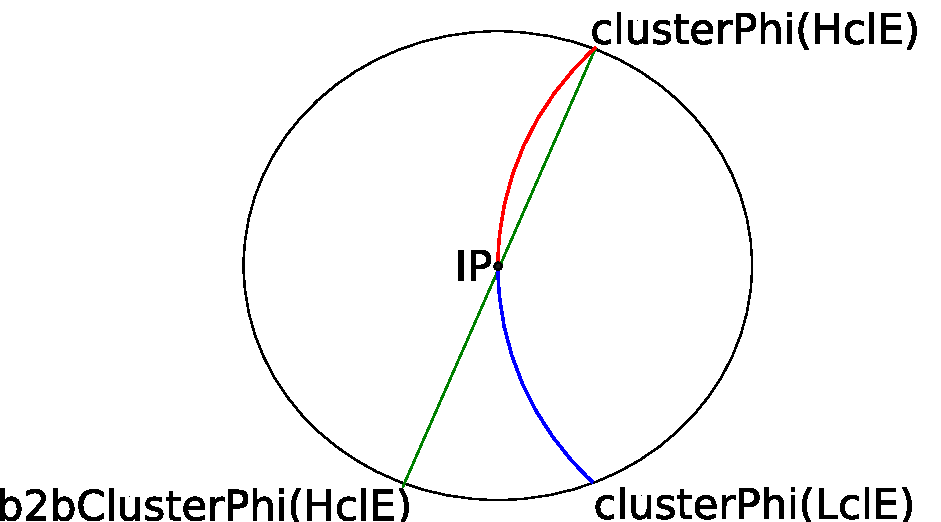
\includegraphics[width=4.5cm]{Plots/b2b_2}
	\end{textblock*}
	
	\begin{textblock*}{0.5\textwidth}(6cm,-3cm)
		\centering
		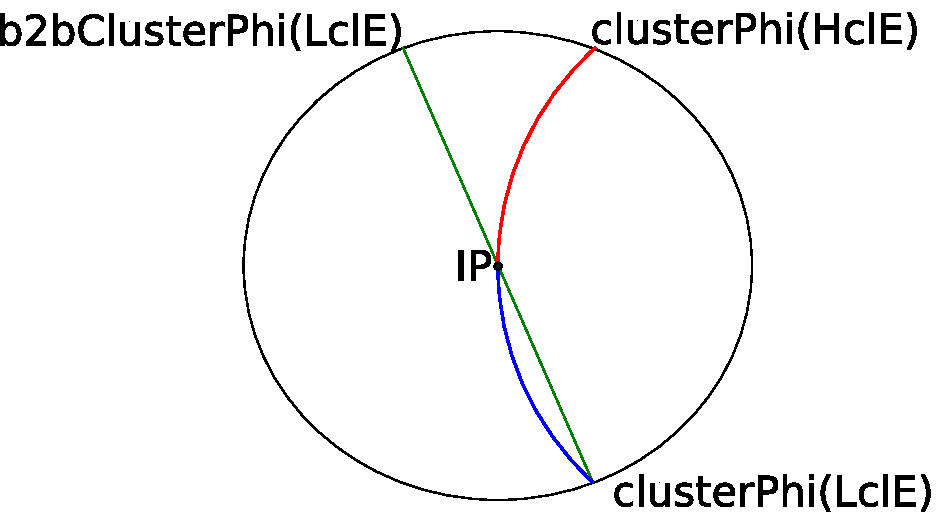
\includegraphics[width=4.5cm]{Plots/b2b_3}
	\end{textblock*}
	
	
	\begin{textblock*}{1\textwidth}(0cm,0.5cm)
		\centering
		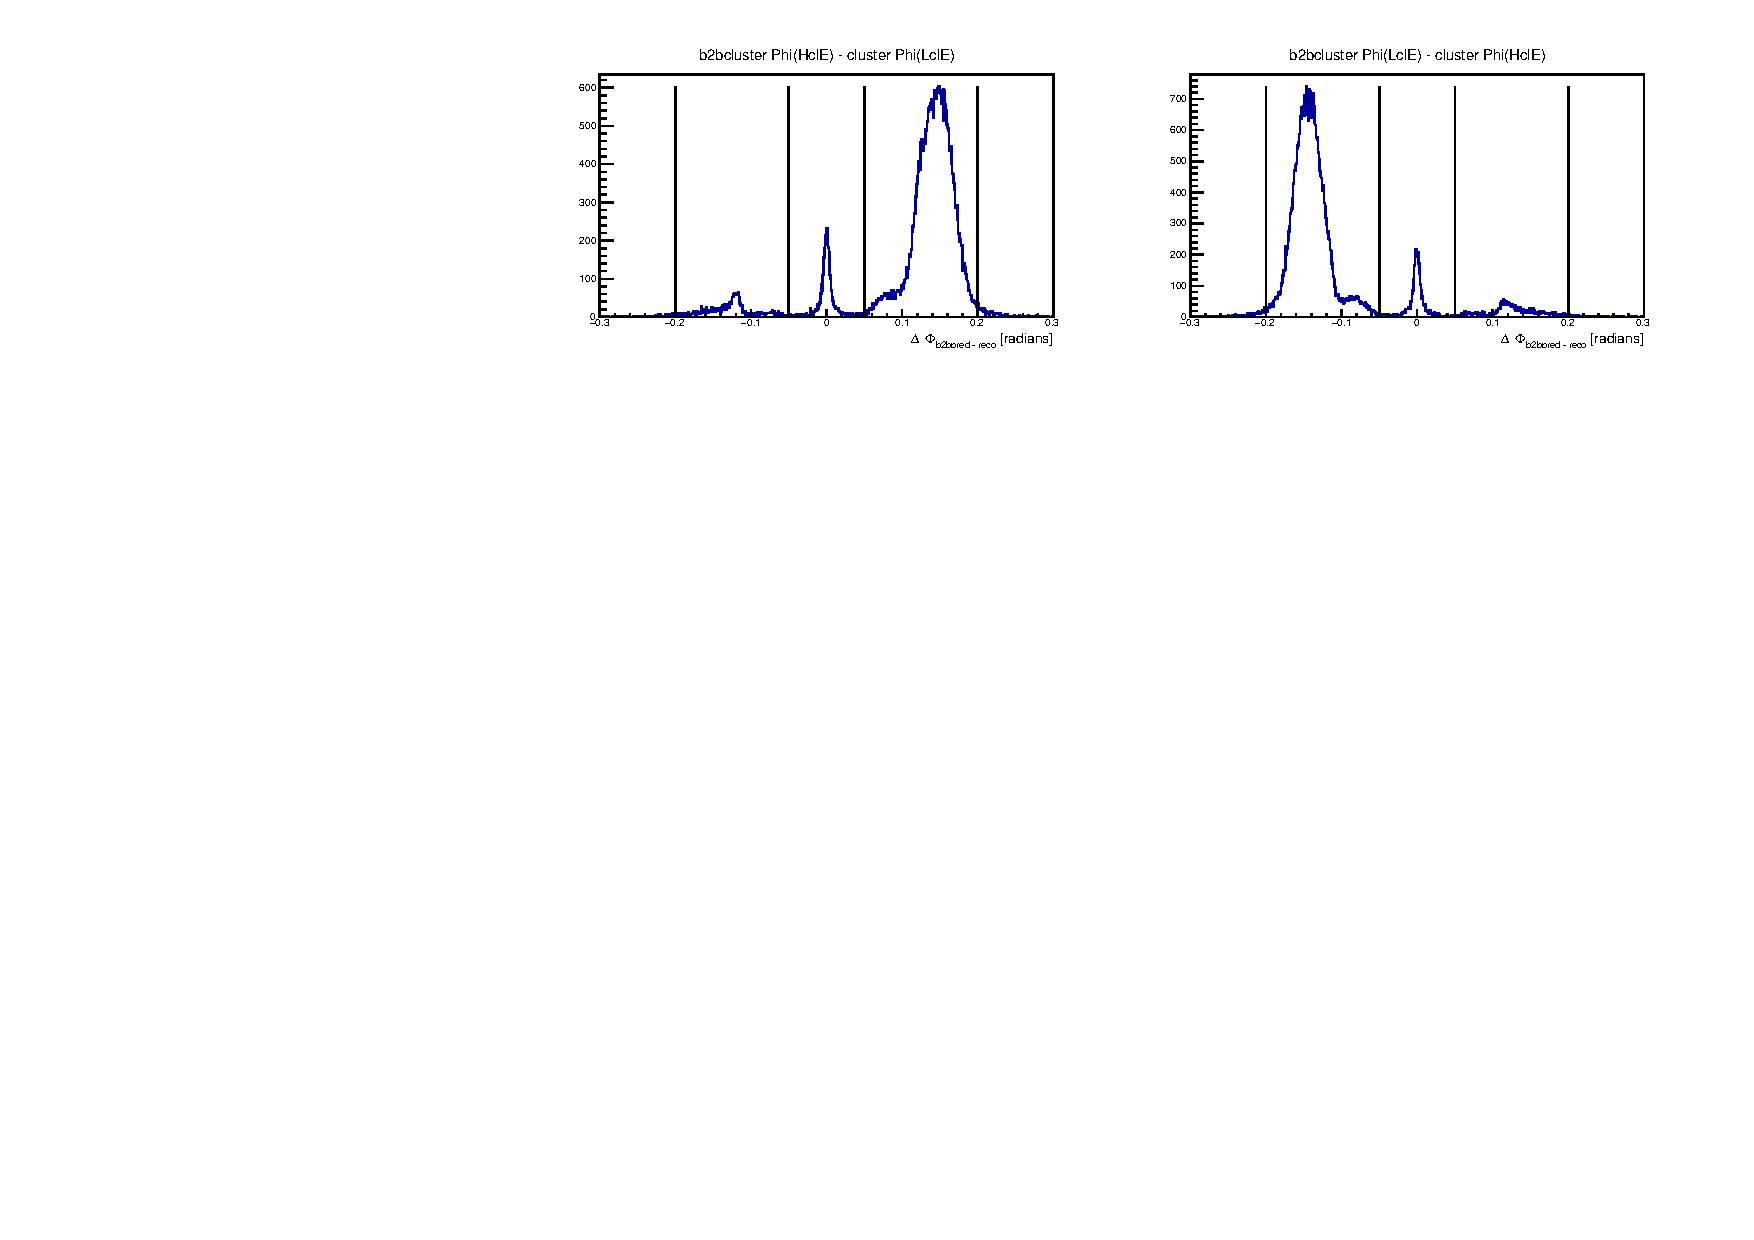
\includegraphics[width=\textwidth]{Plots/Eff/b2b_Data.pdf}
	\end{textblock*}
	
	
	
	

		\begin{textblock*}{0.3\textwidth}(4.cm,0cm)
		\textcolor{blue}{Phase 2 data}		
		\textcolor{blue}{r02608}
	\end{textblock*}
	

	
	
	
	
	
\end{frame}
	
\begin{frame}{Bhabha Event Selection (MC)}	
	
		\begin{textblock*}{0.5\textwidth}(0cm,-3cm)
		\centering
		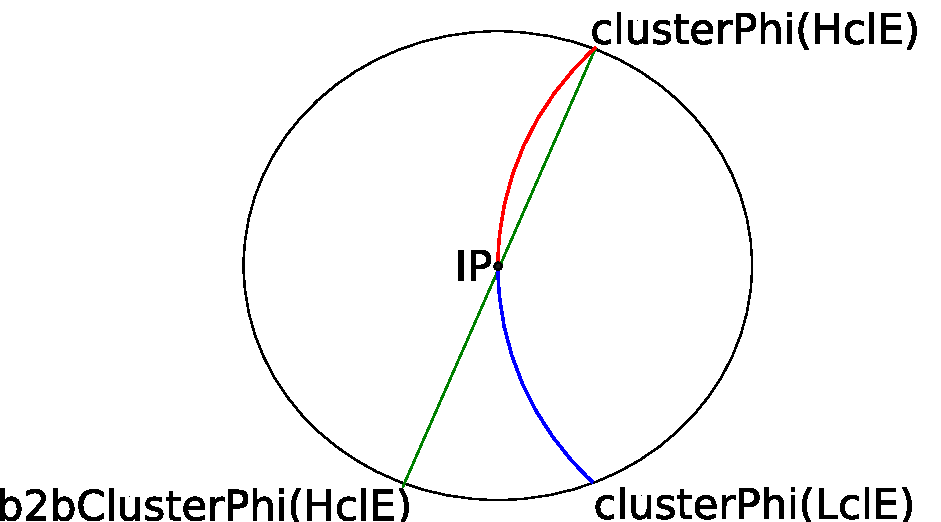
\includegraphics[width=4.5cm]{Plots/b2b_2}
	\end{textblock*}
	
	\begin{textblock*}{0.5\textwidth}(6cm,-3cm)
		\centering
		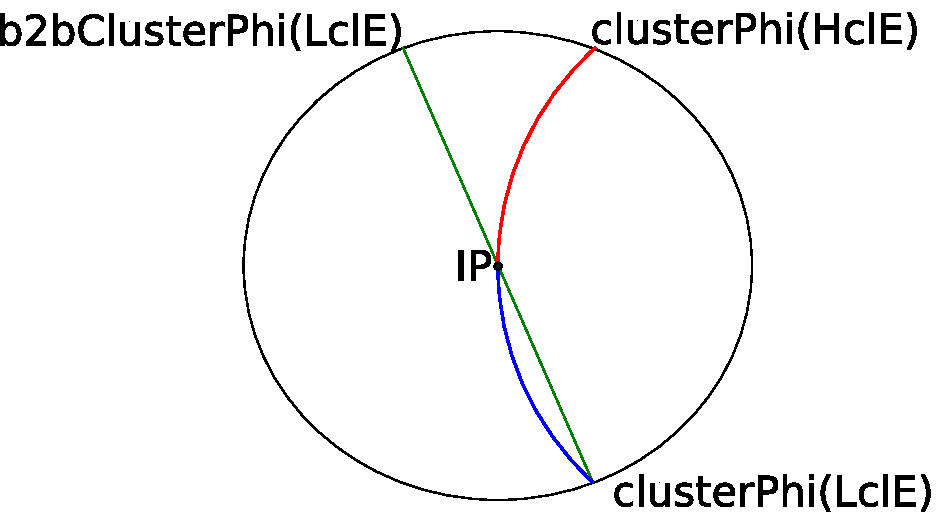
\includegraphics[width=4.5cm]{Plots/b2b_3}
	\end{textblock*}
	

		\begin{textblock*}{1\textwidth}(0cm,0.5cm)
		\centering
		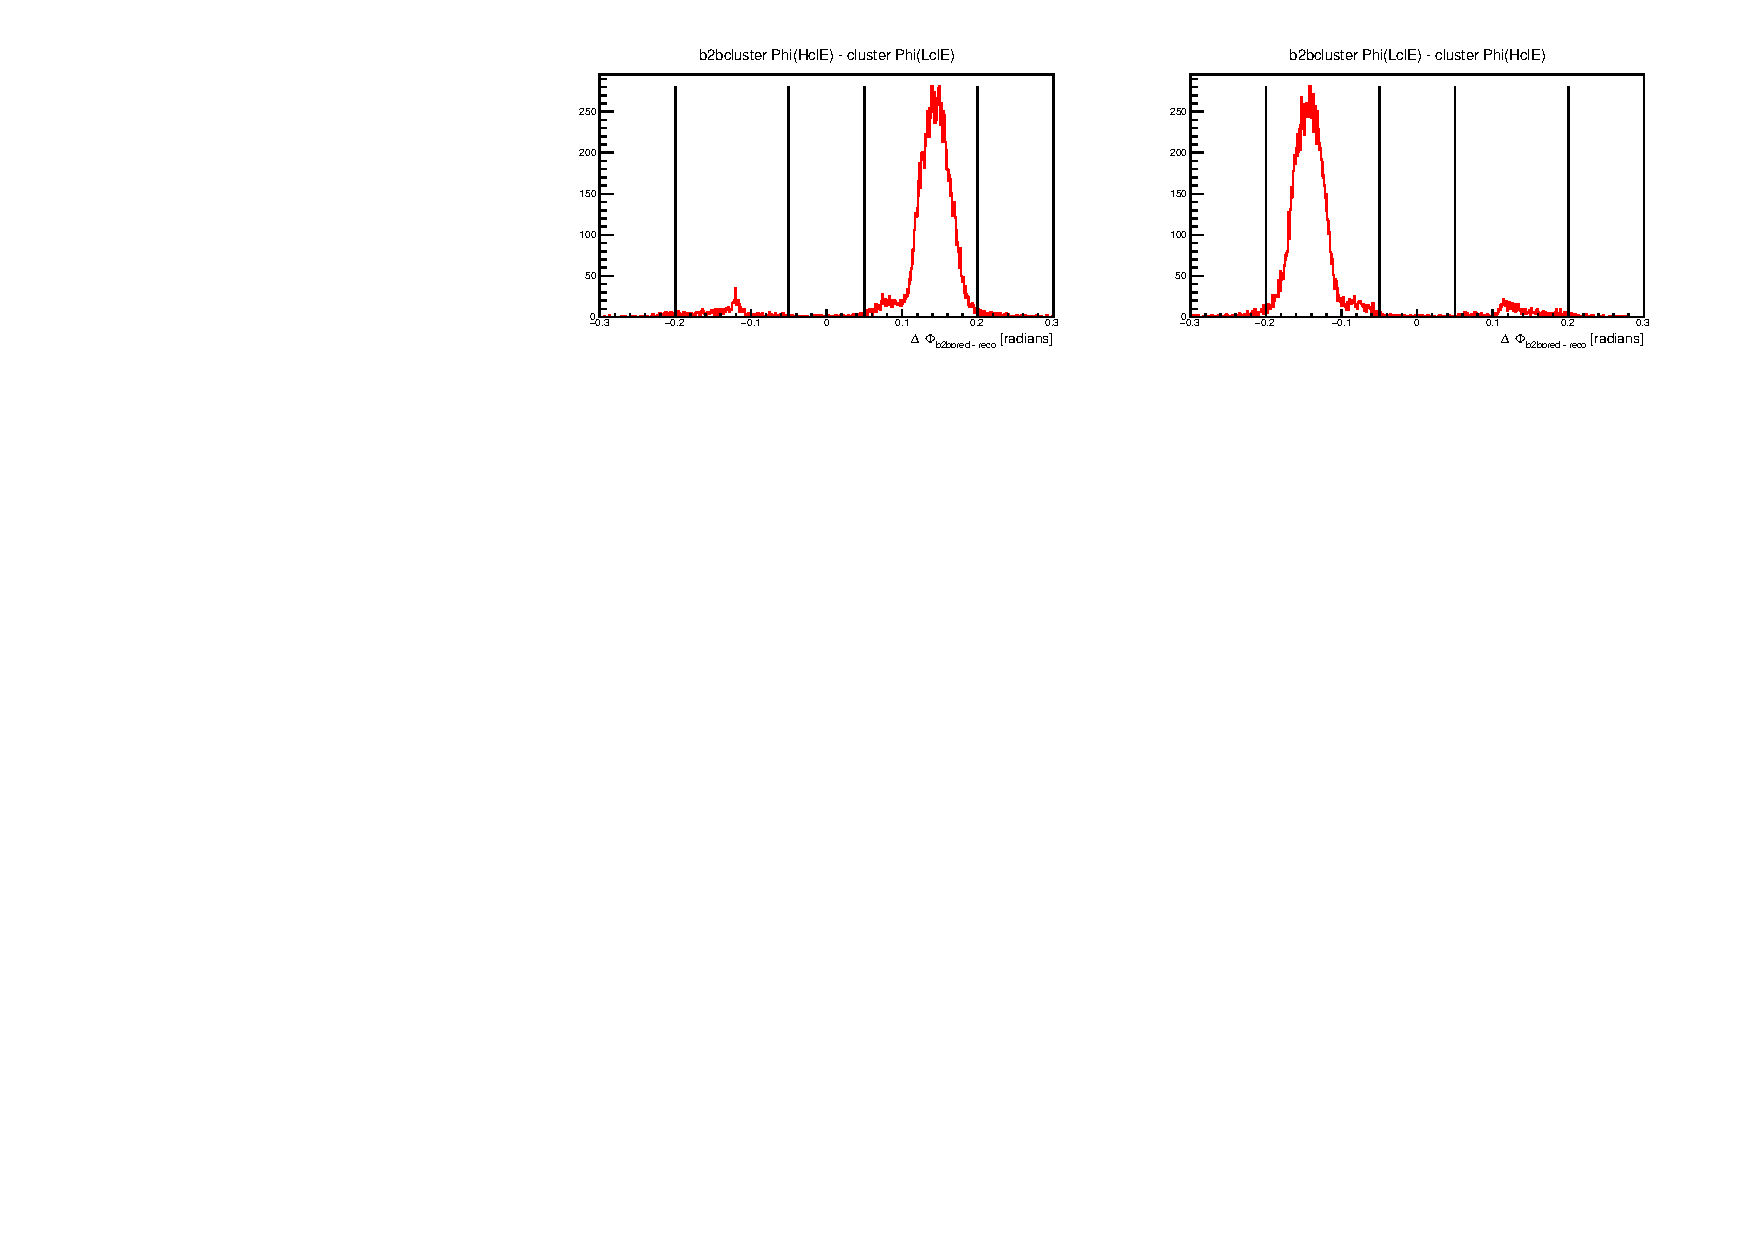
\includegraphics[width=\textwidth]{Plots/Eff/b2b_MC.pdf}
	\end{textblock*}







	\begin{textblock*}{0.3\textwidth}(4.4cm,0cm)
		\textcolor{red}{MC: $\textrm{ee} \rightarrow \textrm{ee}$}
	\end{textblock*}





\end{frame}



\begin{frame}{More Events}
	\textcolor{red}{MC}:
	\begin{itemize}
	
		\item /belle/MC/release-02-00-01/DB00000411/MC11/prod00006731/
		s00/e1002/4S/r00000/3600520000/mdst/sub00
		\item $ 5272146$ candidates selected
	\end{itemize}
	\textcolor{blue}{Phase 2 data}:
	\begin{itemize}
		\item /ghi/fs01/belle2/bdata//Data/release-03-00-03/
		DB00000528/proc00000008/e0003/4S/r02*/all/mdst/sub00/*.root
		\item proc8
		\item $3669759$ candidates selected 
	\end{itemize}

\end{frame}









\begin{frame}{Compare MC And Phase 2 data Efficiency}
	\begin{figure}
		\centering
		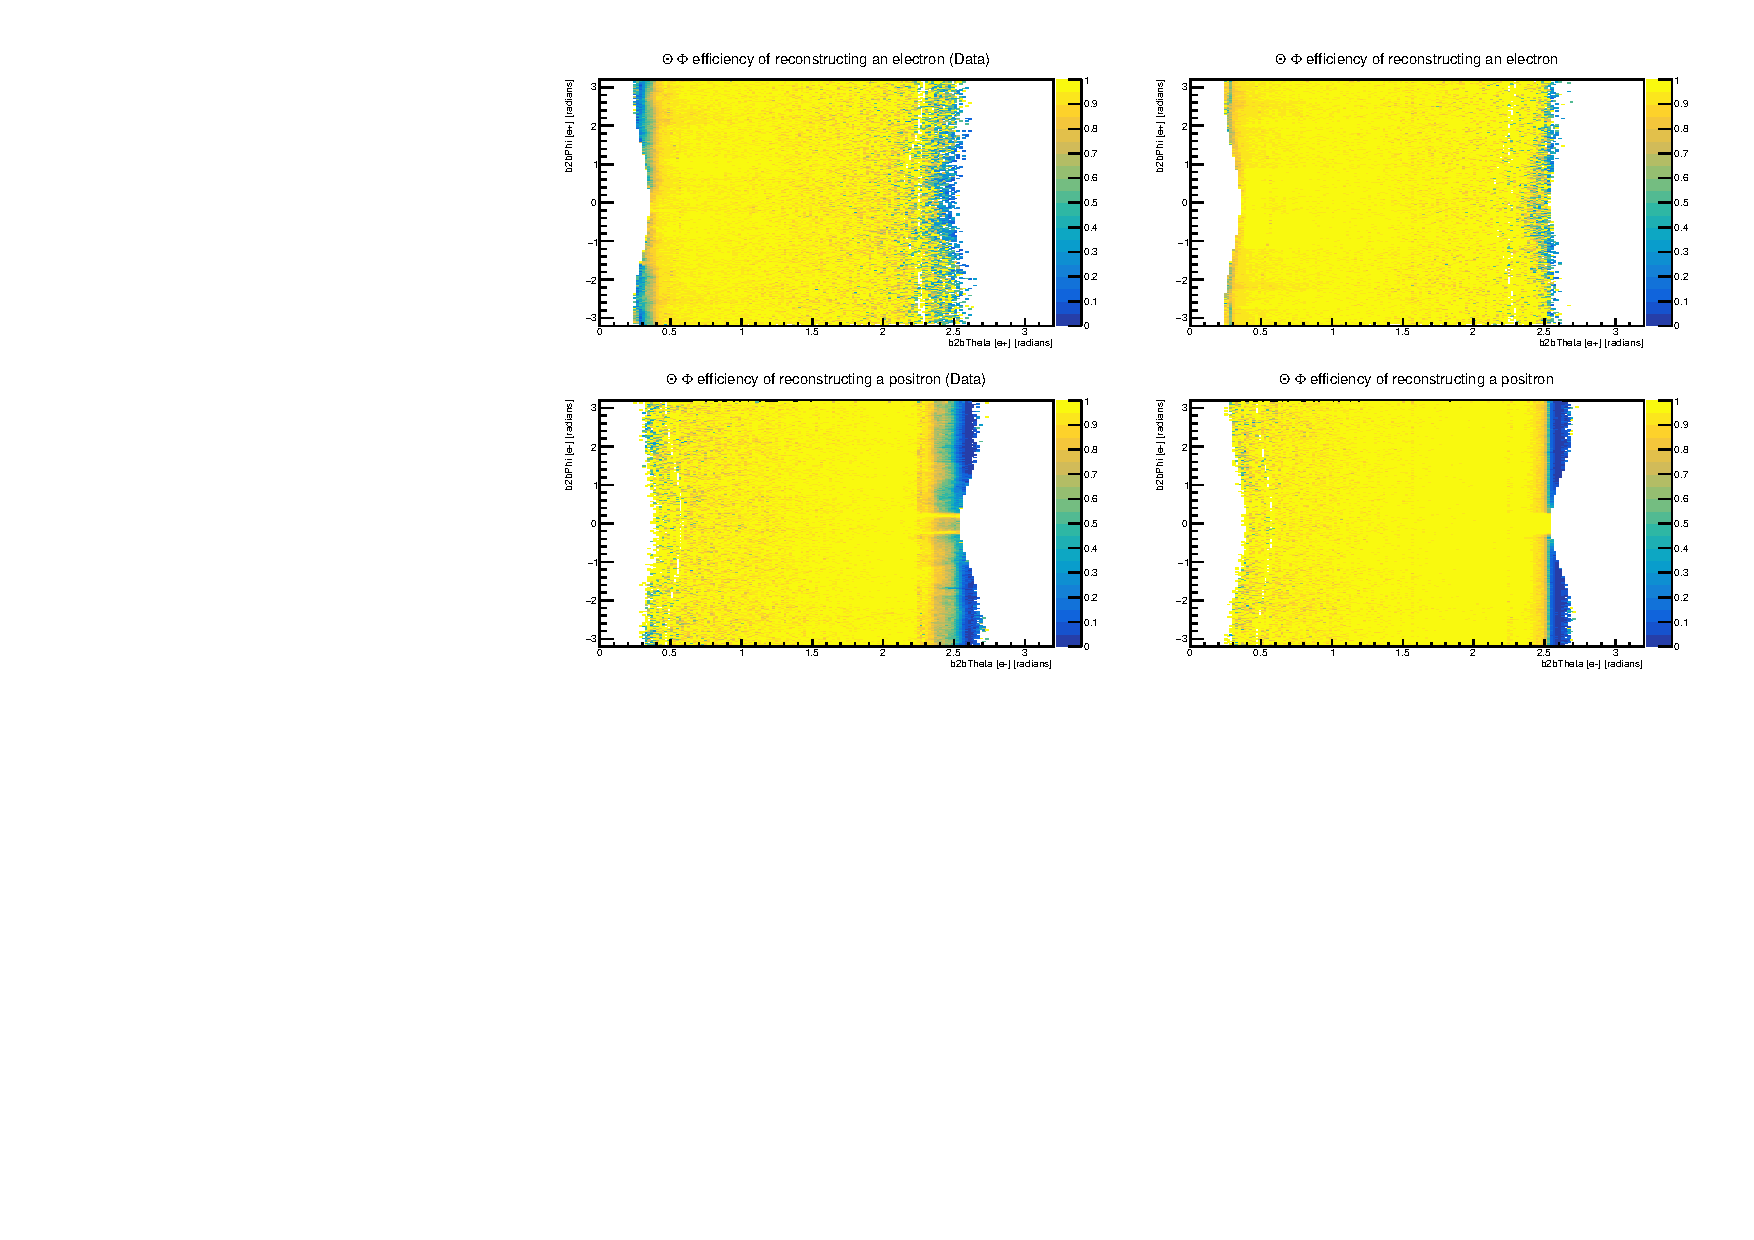
\includegraphics[width=\textwidth]{Plots/Eff/TPMCData}
	\end{figure}

	\begin{textblock*}{0.3\textwidth}(-0.5cm,-5cm)
	$\textrm{e}^-$
\end{textblock*}
\begin{textblock*}{0.3\textwidth}(-0.5cm,-2cm)
	$\textrm{e}^+$
\end{textblock*}


\begin{textblock*}{0.3\textwidth}(1.65cm,-6.7cm)
	\textcolor{blue}{Phase 2 data}
\end{textblock*}


\begin{textblock*}{0.3\textwidth}(7.87cm,-6.7cm)
	\textcolor{red}{MC}
\end{textblock*}



\end{frame}

\begin{frame}{Theta And Phi Projection}
	\begin{figure}
		\centering
		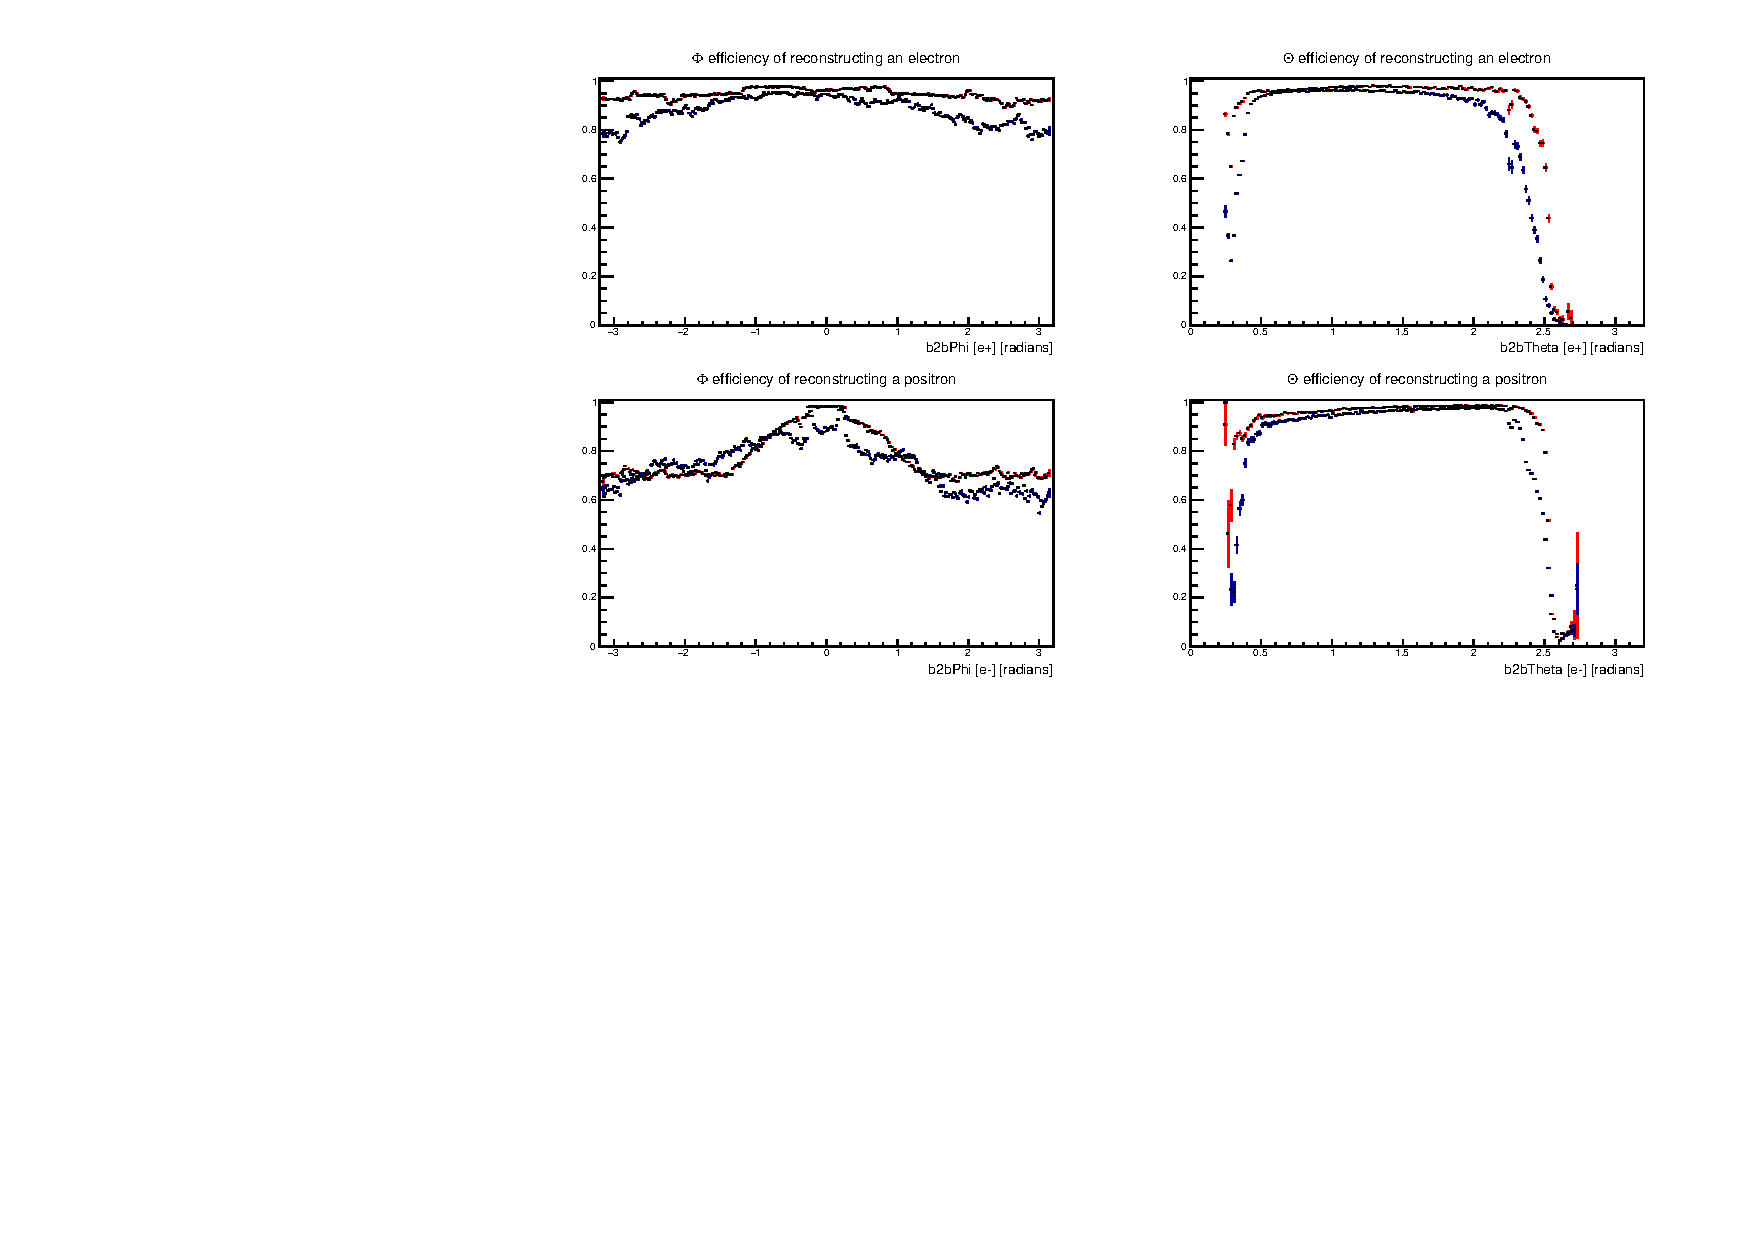
\includegraphics[width=\textwidth]{Plots/Eff/MCDataEff}
	\end{figure}

	\begin{textblock*}{0.3\textwidth}(-0.5cm,-5cm)
		$\textrm{e}^-$
	\end{textblock*}
	\begin{textblock*}{0.3\textwidth}(-0.5cm,-2cm)
		$\textrm{e}^+$
	\end{textblock*}


	\begin{textblock*}{0.3\textwidth}(2.5cm,-6.7cm)
		$\Phi$
	\end{textblock*}


	\begin{textblock*}{0.3\textwidth}(7.87cm,-6.7cm)
	$\Theta$
\end{textblock*}


\begin{textblock*}{0.5\textwidth}(1cm,-5cm)
	\textcolor{blue}{Phase 2 data}
	
	\textcolor{red}{MC}
	
	
\end{textblock*}
	
\end{frame}




\end{document}
